\documentclass[11pt]{article}
\usepackage[margin=1in]{geometry}
\usepackage{tikz}
\usetikzlibrary{shapes.geometric, arrows.meta, positioning, fit, calc}
\usepackage{booktabs}
\usepackage{listings}
\usepackage{xcolor}
\usepackage{hyperref}
\usepackage{amsmath}
\usepackage{enumitem}
\usepackage{fancyhdr}

% Color definitions
\definecolor{codeblue}{RGB}{0,102,204}
\definecolor{codegray}{RGB}{128,128,128}
\definecolor{tablegreen}{RGB}{34,139,34}
\definecolor{tableorange}{RGB}{255,140,0}
\definecolor{tablered}{RGB}{220,20,60}

% Listings configuration
\lstset{
    basicstyle=\ttfamily\small,
    keywordstyle=\color{codeblue},
    commentstyle=\color{codegray},
    breaklines=true,
    frame=single,
    backgroundcolor=\color{gray!5}
}

\hypersetup{
    colorlinks=true,
    linkcolor=codeblue,
    urlcolor=codeblue
}

\pagestyle{fancy}
\fancyhf{}
\rhead{Shire AI}
\lhead{Technical Memo}
\rfoot{\thepage}

\title{\textbf{Shire AI: A Restaurant Intelligence Platform}\\[0.5em]
\large Automated Table Classification, Fairness-First Routing, and AI Scheduling}
\author{Cameron Kuperman \and Harshith Guduru \and Alex Tabaku \and Ben Tang}
\date{\today}

\begin{document}
\maketitle

\section{Executive Summary}

\textbf{Problem.} Restaurant operations traditionally rely on manual monitoring of table states, subjective waiter assignments, and time-consuming schedule creation. These inefficiencies lead to inconsistent customer experiences, unfair tip distribution among staff, and suboptimal resource utilization.

\textbf{Solution.} We present an integrated ML platform that automates three core operational challenges:

\begin{enumerate}[itemsep=0pt]
    \item \textbf{Table State Classification}: Real-time CCTV analysis classifies tables as \textcolor{tablegreen}{clean}, \textcolor{tableorange}{occupied}, or \textcolor{tablered}{dirty} using deep learning
    \item \textbf{Waiter Routing}: Fairness-first algorithm balances workload and tip distribution while maintaining service efficiency
    \item \textbf{Operational Intelligence}: Data-driven insights for menu pricing, server performance tracking, staff scheduling, and customer review analysis
\end{enumerate}

\textbf{Key Capabilities.}
The system processes video streams at $>$15 FPS, achieving 95\%+ classification accuracy with temporal smoothing. The routing algorithm guarantees no waiter receives less than 50\% of average tips through an ``underserved override'' mechanism. The operational intelligence suite provides menu item scoring, Z-score normalized server performance tiers, Gini-optimized scheduling, and LLM-powered review sentiment analysis.

\section{System Architecture}

\subsection{High-Level Data Flow}

\begin{center}
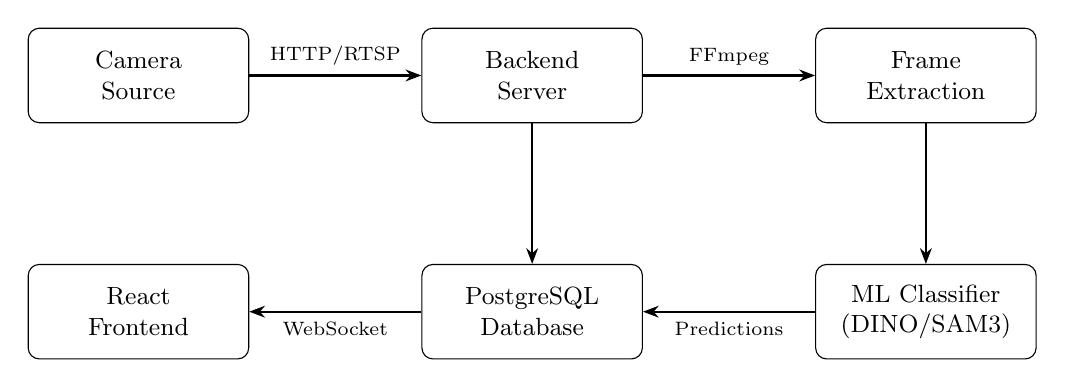
\begin{tikzpicture}[
    node distance=3cm and 5cm, % Increased: first value is vertical, second is horizontal
    on grid,
    box/.style={rectangle, draw, rounded corners, minimum width=2.8cm, minimum height=1.2cm, align=center, font=\small},
    arrow/.style={-{Stealth[length=2mm]}, thick}
]
    % Top row
    \node[box] (camera) {Camera\\Source};
    \node[box, right=of camera] (backend) {Backend\\Server};
    \node[box, right=of backend] (frames) {Frame\\Extraction};

    % Bottom row - explicitly placed below the top row counterparts
    \node[box, below=of camera] (frontend) {React\\Frontend};
    \node[box, below=of backend] (db) {PostgreSQL\\Database};
    \node[box, below=of frames] (ml) {ML Classifier\\(DINO/SAM3)};

    % Horizontal Arrows (Top)
    \draw[arrow] (camera) -- node[above, font=\scriptsize] {HTTP/RTSP} (backend);
    \draw[arrow] (backend) -- node[above, font=\scriptsize] {FFmpeg} (frames);

    % Vertical Arrow (Right Side)
    \draw[arrow] (frames) -- (ml);

    % Horizontal Arrows (Bottom)
    \draw[arrow] (ml) -- node[below, font=\scriptsize] {Predictions} (db);
    \draw[arrow] (db) -- node[below, font=\scriptsize] {WebSocket} (frontend);

    % Vertical Arrow (Middle)
    \draw[arrow] (backend) -- (db);
\end{tikzpicture}
\end{center}

\subsection{Technology Stack}

\begin{center}
\centering
\begin{tabular}{@{}lll@{}}
\toprule
\textbf{Component} & \textbf{Technology} & \textbf{Purpose} \\
\midrule
Backend API & FastAPI + SQLAlchemy & Async REST endpoints, DB access \\
Video Processing & FFmpeg + OpenCV & Frame extraction, crop handling \\
ML Inference & PyTorch + HuggingFace & Table state classification \\
Database & PostgreSQL & State persistence, audit logging \\
Frontend & React + Zustand & Real-time floor plan visualization \\
\bottomrule
\end{tabular}
\end{center}

\section{ML Classification Pipeline}

\subsection{DINOv3 Classifier Architecture}

Our primary classifier leverages a frozen DINOv3 Vision Transformer backbone with a custom attention-pooled classification head:

\begin{center}
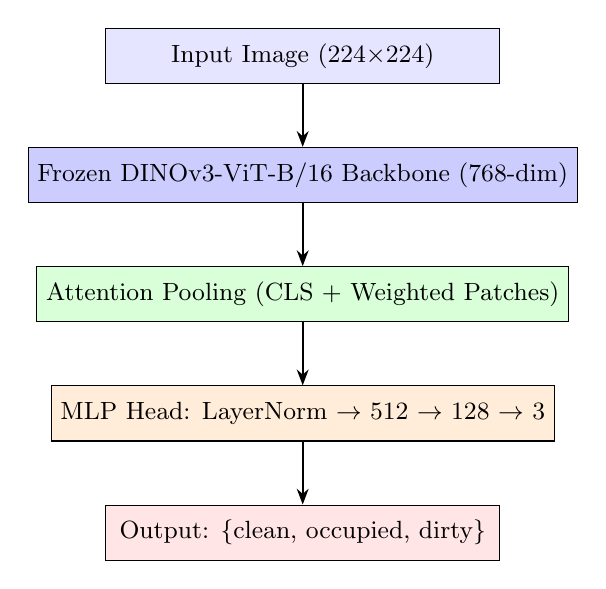
\begin{tikzpicture}[
    node distance=0.8cm,
    block/.style={rectangle, draw, minimum width=5cm, minimum height=0.7cm, align=center, font=\small},
    arrow/.style={-{Stealth[length=2mm]}, thick}
]
    \node[block, fill=blue!10] (input) {Input Image (224$\times$224)};
    \node[block, fill=blue!20, below=of input] (backbone) {Frozen DINOv3-ViT-B/16 Backbone (768-dim)};
    \node[block, fill=green!15, below=of backbone] (pool) {Attention Pooling (CLS + Weighted Patches)};
    \node[block, fill=orange!15, below=of pool] (mlp) {MLP Head: LayerNorm $\rightarrow$ 512 $\rightarrow$ 128 $\rightarrow$ 3};
    \node[block, fill=red!10, below=of mlp] (output) {Output: \{clean, occupied, dirty\}};

    \draw[arrow] (input) -- (backbone);
    \draw[arrow] (backbone) -- (pool);
    \draw[arrow] (pool) -- (mlp);
    \draw[arrow] (mlp) -- (output);
\end{tikzpicture}
\end{center}

\textbf{Technical Novelties:}

\begin{enumerate}[itemsep=2pt]
    \item \textbf{Group-Based Data Splitting}: Consecutive CCTV frames are highly correlated. We group by session+timestamp+table using \texttt{GroupShuffleSplit} to ensure train/val/test sets are truly independent, preventing data leakage.

    \item \textbf{Learned Attention Pooling}: Rather than using only the CLS token, we learn which image patches are discriminative via: Linear(768$\rightarrow$128) $\rightarrow$ Tanh $\rightarrow$ Linear(128$\rightarrow$1) $\rightarrow$ Softmax. This focuses on plates, dishes, and people rather than background.

    \item \textbf{Imbalanced Data Handling}: We combine inverse-frequency class weights, Focal Loss $(1-p)^\gamma \cdot \text{CE}$ with $\gamma=2.0$, WeightedRandomSampler, and Mixup augmentation ($\alpha=0.2$).
\end{enumerate}

\subsection{SAM3 Zero-Shot Alternative}

For deployment without training data, we offer a Segment Anything Model 3 classifier using text-prompted segmentation:

\begin{lstlisting}[language=Python]
if detect("person") and mask_area > 10%: return "occupied"
elif detect("plate") and mask_area > 0.5%: return "dirty"
else: return "clean"
\end{lstlisting}

\subsection{Temporal Smoothing}

To reduce classification jitter, we implement \textbf{N-frame consensus}: states only change when the last $N$ frames (default: 5) all agree on the new classification.

\section{Waiter Routing Algorithm}

\subsection{Fairness-First Scoring}

The routing algorithm balances efficiency with fairness using a priority formula:

\begin{equation}
\text{priority} = (\text{efficiency} \times w_e) - \left(\frac{\text{tables}}{\text{max\_tables}} \times w_w\right) - \left(\frac{\text{waiter\_tips}}{\text{total\_tips}} \times w_t\right) - \text{recency}
\end{equation}

\begin{table}[h]
\centering
\begin{tabular}{@{}llp{6cm}@{}}
\toprule
\textbf{Factor} & \textbf{Weight} & \textbf{Purpose} \\
\midrule
Efficiency Score & $w_e = 1.0$ & Composite: turn time (0.3), tip \% (0.4), covers (0.3) \\
Workload Penalty & $w_w = 3.0$ & Prevents overloading any single waiter \\
Tip Penalty & $w_t = 2.0$ & Ensures fair tip distribution across staff \\
Recency Penalty & 1.5 & Soft no-double-seat (decays over 5 min) \\
\bottomrule
\end{tabular}
\end{table}

\textbf{Underserved Override}: If a waiter has $<$50\% of average covers \textit{and} $<$50\% of average tips, the recency penalty is waived. This guarantees no staff member is systematically disadvantaged.

\section{Operational Intelligence Suite}

\subsection{Review Intelligence}

Multi-platform scraping feeds ByteDance Seed 1.6 for 5-category sentiment analysis (e.g., food, service), automatically flagging reviews that require manager attention.

\subsection{Menu Intelligence}

Items are ranked by a composite score:
\begin{equation}
\text{score} = (\text{orders/day})_{\text{norm}} \times 0.5 + \frac{\text{price} - \text{cost}}{\text{price}} \times 0.5
\end{equation}

The system suggests +10--15\% price hikes for high-demand/low-margin items and flags underperformers (score $<25$) for removal.

\subsection{Server Intelligence}

Waiter performance applies Z-score normalization:
\begin{equation}
\text{performance} = 0.3 \cdot z_{\text{turn\_time}}^{-1} + 0.4 \cdot z_{\text{tip\_pct}} + 0.3 \cdot z_{\text{covers}}
\end{equation}

Percentile-based tiers ($\geq$p75 Strong, $<$p25 Developing) drive routing priority and LLM-generated improvement insights.

\subsection{Scheduling Intelligence}

Forecasts use exponential decay ($0.85^{\text{weeks}}$) to feed the assignment algorithm:
\begin{equation}
\text{score} = 0.5 \cdot \text{constraints} + 0.3 \cdot (\text{fairness\_impact} + 50) + 0.2 \cdot \text{preferences}
\end{equation}

Calculations enforce hard constraints and fairness (Gini $<0.25$) while weighting shift preferences. Analytics endpoints support aggregate views and drill-downs.

\section{Live Video Integration with Swann Security}

For real-time annotation and inference on live camera feeds, we integrated directly with Swann security software:

\begin{center}
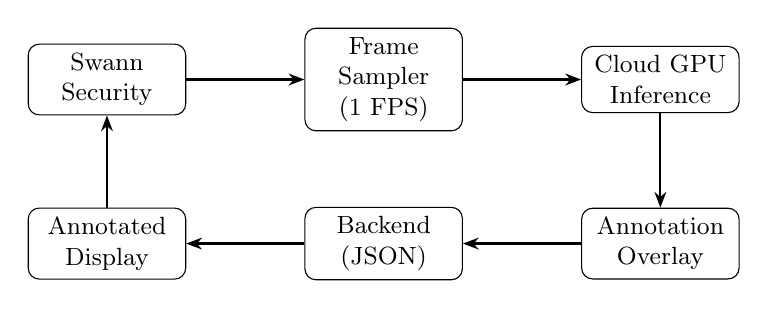
\begin{tikzpicture}[
    node distance=1.2cm and 1.5cm,
    box/.style={rectangle, draw, rounded corners, minimum width=2cm, minimum height=0.8cm, align=center, font=\small},
    arrow/.style={-{Stealth[length=2mm]}, thick}
]
    \node[box] (swann) {Swann\\Security};
    \node[box, right=of swann] (sample) {Frame\\Sampler\\(1 FPS)};
    \node[box, right=of sample] (gpu) {Cloud GPU\\Inference};
    \node[box, below=of gpu] (overlay) {Annotation\\Overlay};
    \node[box, left=of overlay] (backend) {Backend\\(JSON)};
    \node[box, left=of backend] (display) {Annotated\\Display};

    \draw[arrow] (swann) -- (sample);
    \draw[arrow] (sample) -- (gpu);
    \draw[arrow] (gpu) -- (overlay);
    \draw[arrow] (overlay) -- (backend);
    \draw[arrow] (backend) -- (display);
    \draw[arrow] (display) -- (swann);
\end{tikzpicture}
\end{center}

\textbf{Pipeline:}
\begin{enumerate}[itemsep=0pt]
    \item Swann video feeds are sampled at 1 frame per second
    \item Frames are sent to cloud GPU (RunPod) for ML inference
    \item Predictions are overlaid back onto the Swann display
    \item JSON annotations are persisted to the backend for training data collection
\end{enumerate}

This closed-loop system enables both real-time monitoring and continuous collection of labeled training data from production environments.

\section*{Conclusion}

This platform addresses core restaurant operational challenges through five integrated systems: ML-powered table classification, fairness-optimized waiter routing, constraint-aware scheduling, review sentiment analysis, and streamlined performance analytics. The combination of computer vision, NLP, and optimization algorithms creates a comprehensive solution that improves both operational efficiency and staff satisfaction.

\end{document}
